\chapter{Исследование существующих когнитивных архитектур и анализ их недостатков}


Проводится анализ по выявлению существующих недоработок прототипа. 
Выявляются недостатки и преимущества по сравнению с другими моделями искусственного интеллекта.

%Это обзорно-аналитическая глава, в которой требуется отразить:

%\begin{itemize}
	%\item результат изучения различных существующих методов решения задач в рамках проблематики УИРа/диплома (иногда даже в смежных областях), это обзорный аспект, который пишется, в основном, на основе имеющейся литературы или/и программного обеспечения;
	%\item сравнение (с какой-либо определенной целью) этих методов и средств.
%\end{itemize}

%Приведенные ниже названия пунктов являются очень примерными, их состав и структура сильно зависят от специфики конкретной работы.




%Большие отсупы --- это хорошо. Облегчает чтение длинных <<простыней>> текста


%ок
\section{Изучение и анализ существующих когнитивных архитектур}

Одной из наиболее известных когнитивных архитектур является архитектура, 
составленная Jonathan Gratch и Stacy Marsella, что описано в работе \cite{Samsonovich03}.
Цель их исследования - создать общую вычислительную модель механизмов, 
лежащих в основе человеческих эмоций, которая сможет всецело их описать. 
Хотя такая модель может давать объяснение человеческого поведения, 
они рассматривают разработку вычислительных моделей эмоций как 
ключевой объект исследований для искусственного интеллекта, 
который будет способствовать развитию большого количества вычислительных систем,
которые моделируют, интерпретируют или влияют на человеческое поведение. 
На рисунке (Рис. \ref{pic:ris1}) демонстрируется Когнитивно-мотивационно-эмоциональная система.

\begin{figure}[h]
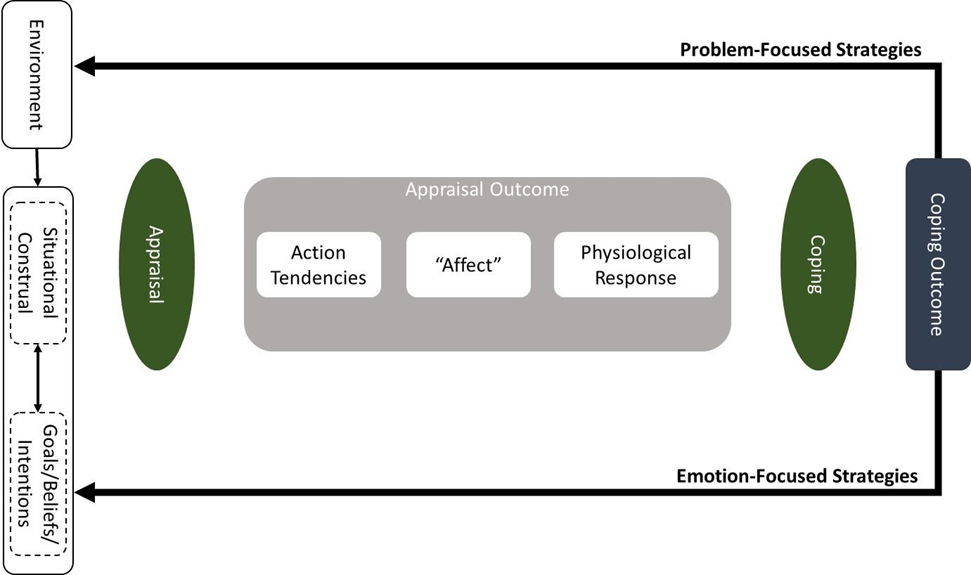
\includegraphics[width=0.75\columnwidth]{./img/ris1.png}
\centering
\caption{Когнитивно-мотивационно-эмоциональная система по материалам Smith and Lazarus.}
\label{pic:ris1}
\end{figure}

Теория оценки служит концептуальной основой их работы, но эта психологическая теория недостаточно точна, чтобы служить
спецификацией вычислительной модели. Для этого они переделывают теорию с точки зрения методов и представлений искусственного интеллекта. 
Когнитивно-мотивационно-эмоциональная система Craig Smith и Richard Lazarus, показанная на рисунке 1, является представителем современных
теорий оценки. Эмоция концептуализируется как двухступенчатая система контроля. Оценка характеризует отношения между человеком и его 
физическим и социальным окружением, называемые отношениями человека и окружающей среды, копирование поведения для восстановления или 
поддержания этих отношений. Поведение возникает в результате тесной связи познания, эмоций и реакций совладения: когнитивные процессы 
служат для построения индивидуальной интерпретации того, как внешние события соотносятся с его целями и желаниями 
(отношения человека и окружающей среды). Система использует эти характеристики для изменения отношений между человеком и окружающей средой,
мотивируя действия, которые изменяют среду (копирование, ориентированное на проблему), или мотивируя изменения в интерпретации этих 
отношений (копирование, ориентированное на эмоции).

Модель PAD была разработана Albert Mehrabian и James A. Russell в 1974 году для описания и измерения эмоциональных состояний, как говорится в Работе \cite{Samsonovich04}. 
В данной модели используются три числовых измерения для представления всех эмоций:
\begin{itemize}
	\item A — arousal (возбуждение);
	\item P — pleasure (удовольствие); 
	\item D — dominance (доминирование).
\end{itemize}

Модель PAD первоначально использовалась в теории психологии окружающей среды, а основное идеей модели было предположение о том,
что физическая среда влияет на людей через их эмоциональное воздействие. На основе данной модели были построены физиологическая 
теория эмоций и теория эмоциональных эпизодов. Также модель использовалась для изучения невербального общения, в потребительском 
маркетинге и при создании анимированных персонажей, которые выражают эмоции.

В модели PAD используются трехмерные шкалы, которые в теории могут иметь любые числовые значения:
\begin{itemize}
	\item шкала удовольствия-неудовольствия показывает, насколько приятно или, наоборот, неприятно человек себя чувствует по отношению к чему-то. Например, радость это — приятная эмоция; гнев и страх — неприятные эмоции;
	\item шкала возбуждения-неактивности измеряет, насколько человек чувствует возбуждение или его отсутствие. В данном случае оценивается именно возбуждение, а не интенсивность эмоций. Например, горе или депрессия характеризуются слабым возбуждением, но сильной интенсивностью; а гнев или ярость имеют и высокую интенсивность, и высокое состояние возбуждения;
	\item шкала доминирования-покорности описывает чувство контроля и доминирования по сравнению со смирением и подчиненностью. Например, гнев — это доминирующая эмоция, а страх
	\item эмоция покорности, хотя обе они имеют неприятный характер.
	\item эмоция покорности, хотя обе они имеют неприятный характер.
\end{itemize}

Еще одна интересная когнитивная архитектура описана в статье трех научных деятелей Ron Sun, Nick Wilson, 
Michael Lynch. Статья имеет название: “Emotion: A Unified Mechanistic Interpretation from a Cognitive Architecture”.
В этой статье рассматривается проект, который пытается интерпретировать эмоции - сложное и многогранное явление с 
механистической точки зрения, чему способствует существующая комплексная вычислительная когнитивная архитектура - CLARION.
Эта когнитивная архитектура состоит из ряда подсистем: подсистем, ориентированных на действие, не ориентированных надействия, 
мотивационной и метакогнитивной подсистем. С этой точки зрения эмоции в первую очередь основаны на мотивации.
Основываясь на этих функциональных возможностях, мы механистически (вычислительно) соединяем части вместе 
в рамках CLARION и фиксируем множество важных аспектов эмоций, как описано в литературе. 
На (Рис. \ref{pic:ris2}) демонстрируются подсистемы когнитивной архитектуры CLARION.
\begin{figure}[h]
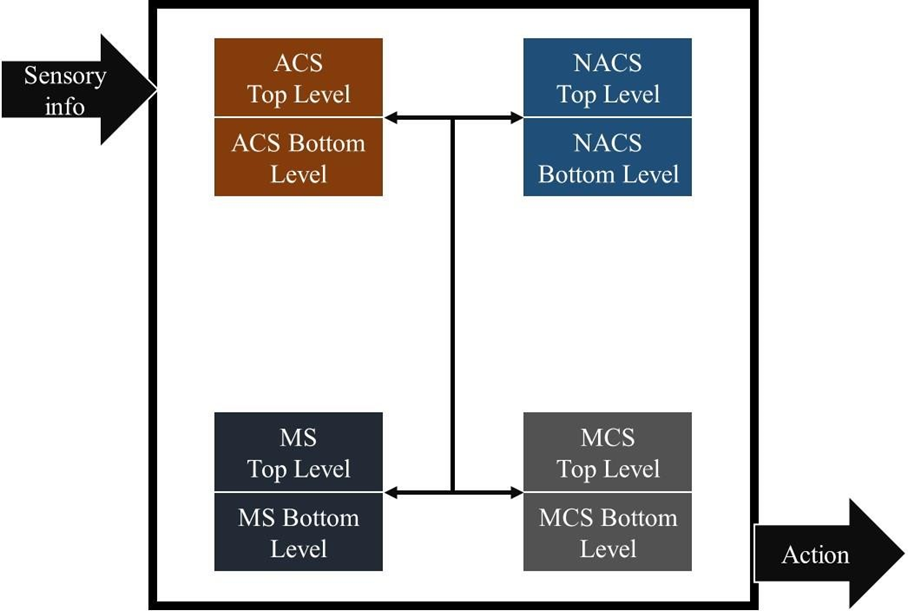
\includegraphics[width=0.75\columnwidth]{./img/ris2.png}
\centering
\caption{Подсистемы когнитивной архитектуры CLARION}
\label{pic:ris2}
\end{figure}

Основные информационные потоки показаны стрелками. ACS означает подсистему, ориентированную на действия. NACS означает подсистему, не ориентированную на действия. МС — это мотивационная подсистема. MCS означает метакогнитивную подсистему.

Получившая наибольшее распространение из всех формальных моделей представления эмоций является модель OCC (Ortony, Clore, \& Collins), 
которая упоминается в работет \cite{Samsonovich06}, 
предложенная в 1988 году учеными Кембриджского университета. Иерархия содержит три ветви, а именно: эмоции, касающиеся последствий 
событий (например, радость и жалость), действия агентов (например, гордость и упрек) и аспекты объектов (например, любовь и ненависть). 
Кроме того, некоторые ветви объединяются в группу сложных эмоций, а именно эмоций относительно последствий событий, вызванных действиями 
агентов (например, благодарность и гнев). 
На рисунке (Рис. \ref{pic:ris3}) демонстрируется оригинальная модель OOC.

\begin{figure}[h]
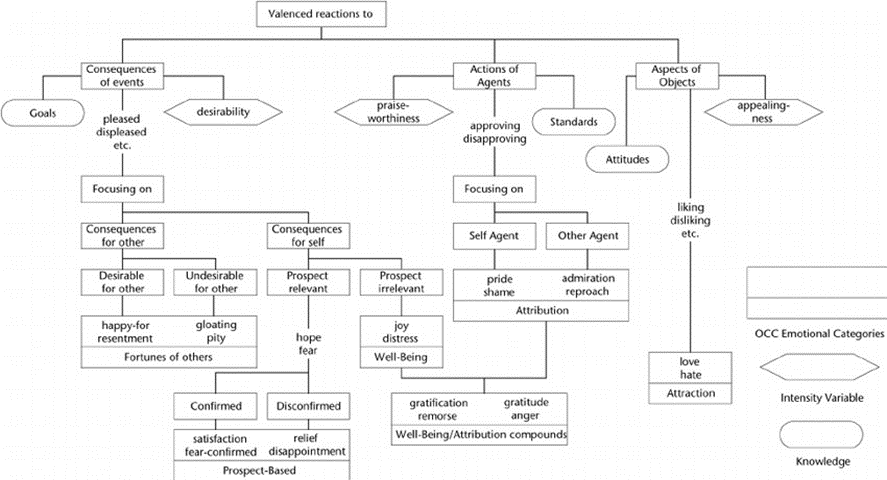
\includegraphics[width=0.75\columnwidth]{./img/ris3.png}
\centering
\caption{Оригинальная модель OCC}
\label{pic:ris3}
\end{figure}
В основе правил динамики данной модели лежит реакция валентности (Valenced reaction). 
Под «валентностью» в психологии понимают внутреннюю привлекательность – «хорошую» 
(положительную валентность) или отвратительность – «плохую» (отрицательную валентность) 
события, объекта или ситуации. Эмоции формируются под воздействием трех основных факторов — 
последствий событий (Consequences of events), действий движущих сил (Actions of agents) и аспектов событий.

Рассмотрим левую «ветку» эмоциональной реакции. Последствия событий могут быть приносящими 
удовольствие (pleased) или доставляющими неудовольствие (displeased). Проведя предварительную 
оценку, человек фокусируется (Focusing on) на разделении последствий событий для себя 
(Consequences for self) и для других (Consequences for self), которые, в свою очередь могут 
оказаться для последних желательными (Desirable for other) или нежелательными (Undesirable for other). 
По поводу судеб других (Fortunes of others) в зависимости от личного отношения — положительного или 
отрицательного — человек может испытывать следующие эмоции: радость за другого (Happy for), 
обида (Resentment), злорадство (Gloating) или жалость (Pity).

У этой модели есть свои ограничения, заключающиеся как в ее требовании упрощения человеческих эмоций,
 так и в ее сложном подходе к тому, как надлежит выводить эмоциональные состояния конечных пользователей 
 посредством интерпретации поведения человека через знаки и сигналы, транслируемые людьми. Использование 
 этой модели в ее оригинальном описании затруднено отсутствием математического аппарата, в следствии чего 
 многие исследователи в своих Виртуальных Акторах используют упрощённые версии данной модели.

Также большой интерес представляет когнитивная архитектура, реализованная в физическом роботе, 
под названием - интегрированное когнитивное универсальное тело (iCub). Это когнитивная архитектура,  
дизайн которой  основан на  существующих знаниях в области робототехники, вычислений, нейробиологии и 
психологии, целью которой является копирование некоторых когнитивных процессов человека для их включения 
в человекоподобных роботов.

Эта архитектура реализована в человекоподобном роботе. Он был разработан для исследования сообществом когнитивных систем. 
Кроме того, он имеет лицензию «Стандартная общественная лицензия GNU (GPL)», так что любой человек может свободно использовать 
все наработки по данному проекту. Данная архитектура реализована в человекоподобном роботе, который имеет 53 степени свободы. 
По размеру он похож на ребенка трех-четырех лет и ребенка в возрасте 2,5 лет по когнитивным способностям. Кроме того, он может 
ползать и сидеть. Некоторые особенности, которые описаны в работе \cite{Samsonovich02}

\begin{itemize}
	\item	Не хватает семантической памяти, чтобы помочь ему обобщать события;
	\item Невозможно сформировать привычки;
	\item Он учится путем подражания, проб и ошибок;
	\item Обнаруживает, распознает и отслеживает человеческое лицо, наблюдая за его действиями; 
	\item Действия основаны на жестах рук, таких как встряхивание и манипулирование объектами,например, толкание, подъем и опускание. 
	\item Действия, наблюдаемые роботом, изучаются и сохраняются в базе данных в процессе обучения.
\end{itemize}

На рисунке (Рис. \ref{pic:ris4}) представлена схема работы iCub.
\begin{figure}[h]
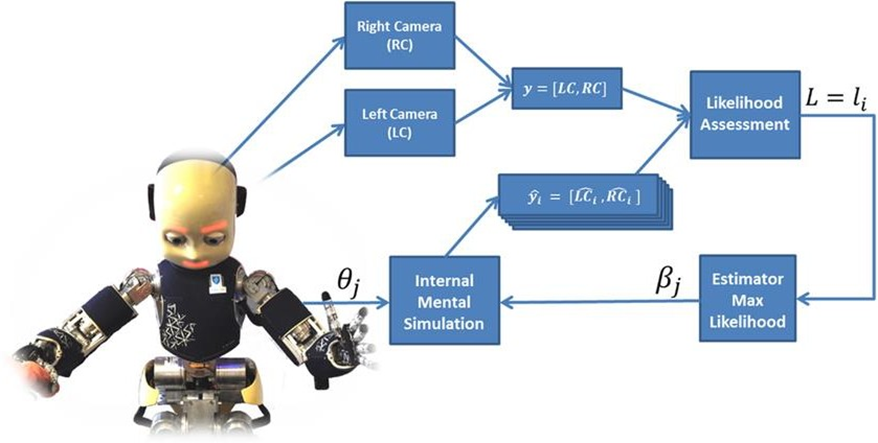
\includegraphics[width=0.75\columnwidth]{./img/ris4.png}
\centering
\caption{Схема работы iCub}
\label{pic:ris4}
\end{figure}

Вспомогательным инструментом при создании актора, наделенного социально- эмоциональным интеллектом, 
может являться - имитация моторного обучения (IML). IML начинает наблюдать за другим актором, осуществляющим 
некоторую цепочку действий, затем категоризирует действия (определяет какую цель преследуют данные действия) 
одновременно отслеживая изменения точки обзора, окружающей среды, положения и типов объектов. Другими словами, 
когда Виртуальный агент неоднократно наблюдает за определенной новой последовательностью действий, каждый из 
знакомых элементов действия активирует соответствующее моторное представление через существующие ассоциации. 
Данное наблюдение формирует связи между элементарными моторными представлениями. Эта связь представлений 
составляет моторное обучение и улучшает имитационное движение. Способность моторной системы интегрировать 
разные части организма позволила бы создать обширный репертуар моторного поведения путем смешивания выходных 
сигналов разных частей организма, чтобы конечный результат отражал относительный и взвешенный вклад каждого в 
достижении цельной имитации движения. Поскольку невозможно воспроизвести функционирование мозга, были созданы 
модели, которые пытаются имитировать различные функции и поведение.
%ок
\section{Изучение и анализ когнитивной архитектуры eBICA}

Архитектура состоит из семи компонентов: интерфейсный буфер, рабочая, процедурная, семантическая 
и эпизодическая системы памяти, система ценностей и система когнитивных карт. Три основных строительных 
блока для этих компонентов — это ментальные состояния, схемы и семантические карты. 
Семантическая память — это коллекция определений схем. Буфер интерфейса заполняется схемами. 
Рабочая память включает активные психические состояния. Эпизодическая память хранит неактивные психические состояния,
сгруппированные в эпизоды - предыдущее содержимое рабочей памяти. Следовательно, эпизодическая память состоит из структур, 
аналогичных тем, которые обнаруживаются в рабочей памяти, но которые «заморожены» в долговременной памяти \cite{seman_karta}. Процедурная 
память включает в себя примитивы. Система ценностей включает в себя шкалы, представляющие основные значения. 
Система когнитивных карт включает, в частности, семантические карты эмоциональных ценностей. 
Семантическая карта использует абстрактное метрическое пространство (семантическое пространство) для представления
семантических отношений между ментальными состояниями, схемами и их 13 экземплярами, а также для присвоения значений их оценкам. 
На (Рис.\ref{pic:ris5}) демонстрируется семантическая карта \cite{seman_karta}.

\begin{figure}[h]
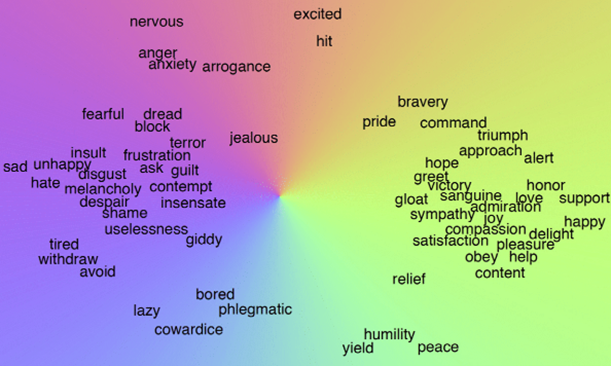
\includegraphics[width=0.75\columnwidth]{./img/ris5.png}
\centering
\caption{Семантическая карта}
\label{pic:ris5}
\end{figure}

Для когнитивного семантического отображения может использоваться слабое когнитивное семантическое картирование. 
Идея заключается в том, чтобы расположить представления на основе очень немногих основных семантических измерениях. 
Эти измерения могут возникать автоматически, если стратегия состоит в том, чтобы объединить синонимы и антонимы друг от друга. 
Карта, часть которой показана на рисунке 6 является результатом этого процесса. Эта карта не очень хорошо отделяет различные 
значения друг от друга: например, основные и сложные чувства. Однако она классифицирует значения в соответствии с их семантикой. 
Рисунок (Рис. \ref{pic:ris6}) демонстрирует примеры простейших эмоциональных элементов в рамках eBICA \cite{Samsonovich01}.

\begin{figure}[h]
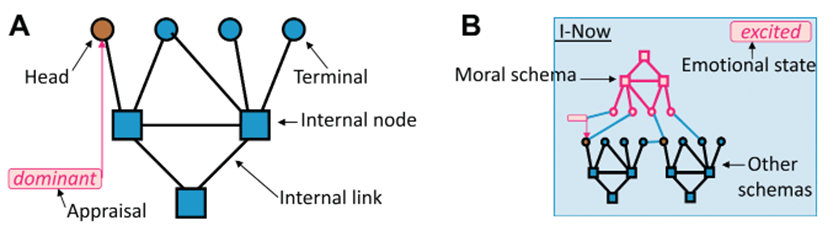
\includegraphics[width=0.75\columnwidth]{./img/ris6.png}
\centering
\caption{примеры эмоциональных элементов в рамках eBICA}
\label{pic:ris6}
\end{figure}

(A) Схема имеет оценку в качестве своего атрибута. Это также атрибут головного узла. Значение этого атрибута - «доминантный», 
что означает, что действие воспринимается как проявление доминирования, или агент воспринимается как «доминантный по отношению ко мне» 
и т. Д. (B) Психическое состояние имеет оценку атрибут, который представляет собой эмоциональное состояние и самооценку агента в данный 
момент в данной ментальной перспективе. Показанная ценность этой оценки «взволнована», что означает, что агент находится в возбужденном 
эмоциональном состоянии. Моральная схема, показанная в B, связывается с частью содержания психического состояния (включая определенный 
образец оценок) и представляет оценку выбранного образца, например, образец взаимодействий и взаимных оценок двух агентов, упомянутых в 
ментальном состоянии.

%можно еще дописать
\section{Нейронные сети и их типы}

Нейро́нная сеть (также искусственная нейронная сеть, ИНС) — математическая модель, а также её программное или аппаратное воплощение, 
построенная по принципу организации и функционирования биологических нейронных сетей — сетей нервных клеток живого организма. 
Это понятие возникло при изучении процессов, протекающих в мозге, и при попытке смоделировать эти процессы. Первой такой попыткой 
были нейронные сети У. Маккалока и У. Питтса. После разработки алгоритмов обучения получаемые модели стали использовать в практических 
целях: в задачах прогнозирования, для распознавания образов, в задачах управления и др. 

Разделяют несколько основных разновидностей Нейронных сетей, согласно работе \cite{neural01}, а именно:
\begin{itemize}
	\item Нейронные сети прямого распространения
	\item Сети радиально-базисных функций
	\item Нейронная сеть Хопфилда (Hopfield network, HN)
	\item Цепи Маркова (Markov chains, MC или discrete time Markov Chains, DTMC)
	\item Машина Больцмана (Boltzmann machine, BM)
	\item Ограниченная машина Больцмана (restricted Boltzmann machine, RBM)
	\item Автокодировщик (autoencoder, AE)
	\item Разреженный автокодировщик (sparse autoencoder, SAE)
	\item Вариационные автокодировщики (variational autoencoder, VAE)
	\item Шумоподавляющие автокодировщики (denoising autoencoder, DAE)
	\item Сеть типа «deep belief» (deep belief networks, DBN)
	\item Свёрточные нейронные сети (convolutional neural networks, CNN)
	\item Развёртывающие нейронные сети (deconvolutional networks, DN)
\end{itemize}

С точки зрения машинного обучения, нейронная сеть представляет собой частный случай методов распознавания образов, дискриминантного анализа.
Рекуррентные нейронные сети (РНС, англ. Recurrent neural network; RNN) — вид нейронных сетей, где связи между элементами образуют 
направленную последовательность \cite{Wikipedia01}. Благодаря этому появляется возможность обрабатывать серии событий во времени или последовательные 
пространственные цепочки. В отличие от многослойных перцептронов, рекуррентные сети могут использовать свою внутреннюю память для 
обработки последовательностей произвольной длины. Поэтому сети RNN применимы в таких задачах, где нечто целостное разбито на части, 
например: распознавание рукописного текста или распознавание речи. Было предложено много различных архитектурных решений для 
рекуррентных сетей от простых до сложных. В последнее время наибольшее распространение получили сеть с долговременной и 
кратковременной памятью (LSTM) и управляемый рекуррентный блок (GRU).

В последнее время наибольшую популярность для решения задач тематической классификации, применяемой для выделения семантического смысла текста,
приобрели глубокие нейронные сети, так как они позволяют достичь наивысшей точности среди всех известных моделей машинного обучения. 
В частности, сверточные нейронные сети совершили прорыв в классификации изображений. В настоящее время они успешно справляются и с 
некоторыми задачами автоматической обработки текстов. Более того, как утверждается в некоторых исследованиях сверточные сети подходят 
для этого даже лучше рекуррентных нейронных сетей, которые чаще всего используются для анализа текстовых последовательностей. 
С другой стороны, использование сверточных сетей для классификации текстов мало исследовано. Поэтому исследование применения 
сверточных нейронных сетей для задачи классификации текстов в качестве альтернативы рекуррентным нейронным сетям представляет 
практический интерес, что описано в \cite{neural10}.

Для решения поставленной задачи требуется получить способ представления данных в виде, пригодном для обработки сверточной нейронной сетью. 
Например, в виде матрицы вещественных чисел. Наиболее распространенным является способ отображения каждого слова в многомерное 
векторное пространство. В рамках данной работы векторные представления слов строились на основе модели word2vec \cite{cyberlinka01}.
sa

\section{Методы определения эмоций в речи}

Для распозавнания эмоций в речи используют следующие подходы:
\begin{itemize}
	\item Анализ эмотивной сотсавляющей текста в речи
	\item Анализ тональности речи
\end{itemize}


На текущий момент сущестуют следующие методы определения тональности текста:
\begin{enumerate}
  \item Анализ текста методами векторного анализа (часто с применением n-граммных моделей), сравнение с ранее размеченным эталонным корпусом по выбранной мере близости и отнесение (классификация) текста к негативу или позитиву на основании полученного результата сравнения.
  \item Поиск эмотивной лексики (лексической тональности) в тексте по заранее составленным тональным словарям (спискам паттернов) с применением лингвистического анализа. По совокупности найденной эмотивной лексики текст может быть оценен по шкале, отражающей количество негативной и позитивной лексики. Этот метод может использовать как списки паттернов, подставляемые в регулярные выражения, так и правила соединения тональной лексики внутри предложения
  \item Смешанный метод (комбинация первого и второго подходов).
\end{enumerate}

% тут надо нормально проставить cit
Первый метод (см., например, [Pang & al., 2002; Pang & al., 2005; Gamon,
2004]) работает достаточно быстро, но требует наличия предварительно размеченного эталонного корпуса, на основе которого происходит обучение алгоритма сравнения. 
Существенными недостатками такого подхода оказываются увеличение трудоемкости и ограничение разнородности корпуса (т. е.
неполнота лексического покрытия), что приводит к потере точности. К тому же
данный метод не позволяет провести глубокий анализ текста, то есть выявить
и показать эмотивность на уровне предложения.
% тут надо нормально проставить cit

Второй метод [Nasukawa, 2003; Yi, 2003] не менее трудоемок в составлении тональных словарей (или получения списка тональных паттернов),
Метод определения эмоций в текстах на русском языке 513
но в сочетании с синтаксическим и морфологическим анализом более гибок:
он позволяет не только показать цепочки тональной лексики, но и получить
синтаксически корректные эмоциональные выражения. При хорошем наполнении тональных словарных списков этот метод позволяет достичь хорошей
полноты (покрытия эмотивной лексики).
% тут надо нормально проставить cit
Недостаток этого метода в том, что с помощью него сложно дать количественную оценку негативности-позитивности текста. 
Чтобы избежать недостатков первого и второго метода, используют смешанный подход [Prabowo &
al., 2009; Konig, 2006], частично включающий в себя два первых.

Следующий метод определения эмоций в речи это их распознавание, посредством акустического анализа.

Индивидуальность голоса обеспечивается сочетанием поведенческих и
физиологических признаков. К поведенческим относят семантику, дикцию,
произношение, ритм, интонации и др. Они обусловлены социальными факто-
рами и могут быть довольно изменчивыми в зависимости от ситуации. Более
надежными являются анатомические особенности речевого тракта, поэтому
для работы автоматического распознавания наиболее адаптированы алгорит-
мы измерения акустических характеристик.

Акустическая теория речи рассматривает речевую волну как результат ра-
боты источника звука и фильтров. Подробное изложение о физиологических
процессах речеобразования и моделях речевого тракта можно найти в кни-
гах [2–4]. Здесь же кратко приведены только те параметры, которые участву-
ют в автоматическом распознавании дикторов.
Характерные черты голоса конкретного человека в цифровой обработке
сигналов получают через спектральный анализ речевой волны.

Частота первой гармоники спектра является частотой основного тона
(основной частотой голоса). Частота основного тона F0 – обратная величина
длительности T0 одного цикла работы голосовых связок: F0 = 1/ T0 . Основная
частота определяет высоту голоса – ощущение, связанное с воздействием тона
на слуховую систему человека.
Индивидуальность данного параметра объясняется тем, что длительность
T0 зависит от массы и упругости голосовых связок, а также от перепада дав-
ления над и под связками. Поэтому пол и возраст диктора оказывают влияние
на значения основной частоты.
Каждый человек имеет свой диапазон изменений частоты основного тона.
Как правило, для взрослого он составляет от полутора до двух октав. В задаче
распознавания личности по голосу необходимо определять базовую основную
частоту, т. е. привычный и удобный для идентифицируемого человека режим
работы голосовых связок.

\section{Классификации и определение эмоций}

Многообразие эмоций, их качественных и количественных проявлений исключают возможность простой и единой классификации. 
Каждая из характеристик эмоций может выступать в качестве самостоятельного критерия, основания для их классификации (таб. \ref{tbl:text_a00}).

\begin{table}[H]
\caption{характеристики эмоции как основания для их классификации}
\label{tbl:text_a00}
\begin{center}
%\centering

\begin{tabular}{ | c | c | }
	\hline
	Знак & Пололожительные, отрицательные, амбивалентные \\ \hline 
	Модальность & Радость, гнев, страх и др. \\ \hline
	Влияение на поведение и деятельность & Осознаваемые, неосознаваемые \\ \hline
	Предметность	& Предметные, беспредментные \\ \hline
	Степень произвольности & Произвольные, непроизвоольные \\ \hline
	Происхождение и развлечения & Врожденные, приобретенные, первичные, вторичные \\ \hline
	Уровень & Высшие, низшие \\ \hline
	Длительность & Кратковременные, длительные \\ \hline
	Интенсивность & Слабые, сильные \\ \hline
\end{tabular}
\end{center}
\end{table}

По знаку эмоциональные переживания можно разделить:
\begin{enumerate}
	\item на положительные
	\item отрицательные
	\item амбивалентные
\end{enumerate}

Основной функцией положительных эмоций является поддержание контакта с позитивным событием, поэтому им присуща реакция приближения к полезному, 
необходимому стимулу. Кроме того, по мнению П.В. Симонова, они побуждают нарушать достигнутое равновесие с окружающей средой и искать новую стимуляцию.

Для отрицательных эмоций характерной является реакция удаления, прерывания контакта с вредным или опасным стимулом.
Считается, что они играют более важную биологическую роль, поскольку обеспечивают выживание индивида.

Амбивалентными эмоциями являются противоречивые эмоциональные переживания, связанные с двойственным отношением к чему-либо или кому-либо (одновременное принятие и отвержение).

\section{Выводы}

Были изучены и проанализированы основные когнитивные архитектуры, особое внимание уделялось когнитивной архитектуры eBICA.
Была рассмотрена проблема синтеза и распознавание речи. Были изучены материалы описывающие классификацию и определение эмоций.

